\section{Introduction}
\label{sec:wowmom-intro}

The RF spectrum is a limited natural resource in great demand due to the
unabated increase in mobile (and hence, wireless) data
consumption~\cite{Jeffrey14,sigcomm21-5G}.
In 2020, the U.S. FCC moves to free up 100 MHz of previously military-occupied mid-band spectrum in the 3.45-3.55 GHz band for paving the way for 5G development. 
Also, the research and industry communities have been addressing this capacity crunch via the development of {\em shared spectrum}.
Spectrum sharing is the simultaneous usage of a specific frequency band in a specific geographical area and time by a number of independent entities where harmful electromagnetic interference is mitigated through agreement (i.e., policy, protocol)~\cite{dod20-spectrum}. 
Spectrum sharing techniques are also normally used in 5G networks to enhance spectrum efficiency~\cite{survey-specshare}.~However, protection of spectrum from unauthorized
users is important in maximizing spectrum utilization.

The increasing affordability of the software-defined radio (SDR)
technologies makes the shared spectrum particularly prone to
unauthorized usage or security attacks. With easy access to SDR
devices (e.g. HackRF, USRP), it is easy for selfish users to transmit data
on a shared spectrum without any authorization and potentially cause
harmful interference to the incumbent users.  Such illegal spectrum
usage could also happen as a result of the infiltration of computer viruses
or malware on SDR devices.~\cite{survey-specshare} depicts three cases of spectrum attack.
As the fundamental objective behind such
shared spectrum paradigms is to maximize spectrum utilization, the
viability of such systems depends on the ability to effectively guard
the shared spectrum against unauthorized usage.  The current
mechanisms however to locate such unauthorized users (intruders) are
human-intensive and time-consuming, involving the FCC enforcement bureau
which detects violations via complaints and manual
investigation~\cite{mobicom17-splot}. 
Motivated by the above, we seek an effective
technique that is able to accurately localize multiple simultaneous
intruders (transmitters). Below, we describe the multiple transmitter localization problem.

%%% Multi-tx and challenges.
\para{Multiple Transmitter Localization (\mtl).}  \eat{Localization of
unauthorized users in a shared spectrum system essentially boils down to localizing transmitters/intruders in a given area under a shared spectrum system.}
The transmitter localization problem has been well studied, but most of the focus has been on localizing a {\em single} transmitter at a time. 
However, it is important to localize multiple transmitters simultaneously to effectively guard a shared spectrum
system. E.g., a malware or virus-based attachment could simultaneously 
cause many devices to violate spectrum allocation rules; spectrum
jamming attacks would typically involve multiple transmitters. More
importantly, a technique limited by the localization of a single intruder
could then be easily circumvented by an offender by using multiple
devices. The key challenge in solving the multiple transmitter localization (\mtl) 
problem comes from the fact that
the deployed sensor would receive only a {\em sum} of the signals from multiple transmitters, and separating the signals may be impossible. 
\eat{In
addition, the other challenge that \mtl in the context of shared
spectrum system poses is the presence of authorized users---e.g., the
incumbent users and the dynamic set of secondary users that have been
allocated spectrum by the manager.}
% To the best our knowledge, no prior localization work has considered the presence of authorized users.

%%%% SPLOT and shortcomings.
\softpara{Prior Works.}
The \mtl problem has been recently addressed in a few prior works, among which \splot~\cite{mobicom17-splot}, \map~\cite{ipsn20-mtl}, and 
\deeptx~\cite{icccn20-deeptxfinder} are the most 
prominent. \splot essentially decomposes the \mtl
problem to multiple single-transmitter localization problems based on
the sensors with the highest power readings in a
neighborhood. However, their technique implicitly assumes a propagation model, and
thus, may not work effectively in areas with complex propagation
characteristics, and it is not effective in the case of transmitters
being located close by (a key challenging scenario for \mtl problem).
Our recent work \map solves the \mtl problem using a 
hypothesis-driven Bayesian approach; in particular, it uses prior training in the form of distributions
of sensor readings for various transmitter locations, and uses the training data to determine
the most likely configuration (i.e., transmitters' locations and powers) for a 
given vector of sensor readings. 
However, to circumvent the high computational cost of a pure Bayesian approach,
\map uses a divide and conquer heuristic which results in somewhat 
high number of misses and false alarms while still incurring high
latency. 
%%%%%%%%%%%
\deeptx uses a CNN-based learning model approach; 
however, they use a separate CNN model for a specific number of transmitters
and thus may incur high model complexity and training costs while also limiting the number 
of transmitters that can be localized.
In our evaluations, we compare our work with each of the above approaches.
%In this approach, like ours, a model is trained, which later is used to predict the configuration of the transmitters the best based on sensors received power.
%\eat{In our evaluation, we
%  have compared our technique with theirs and one other approach.}
%%\blue{Our localization approach belongs to the fingerprinting~\cite{infocom00-radar} category.}

\begin{figure}[t]
\centering
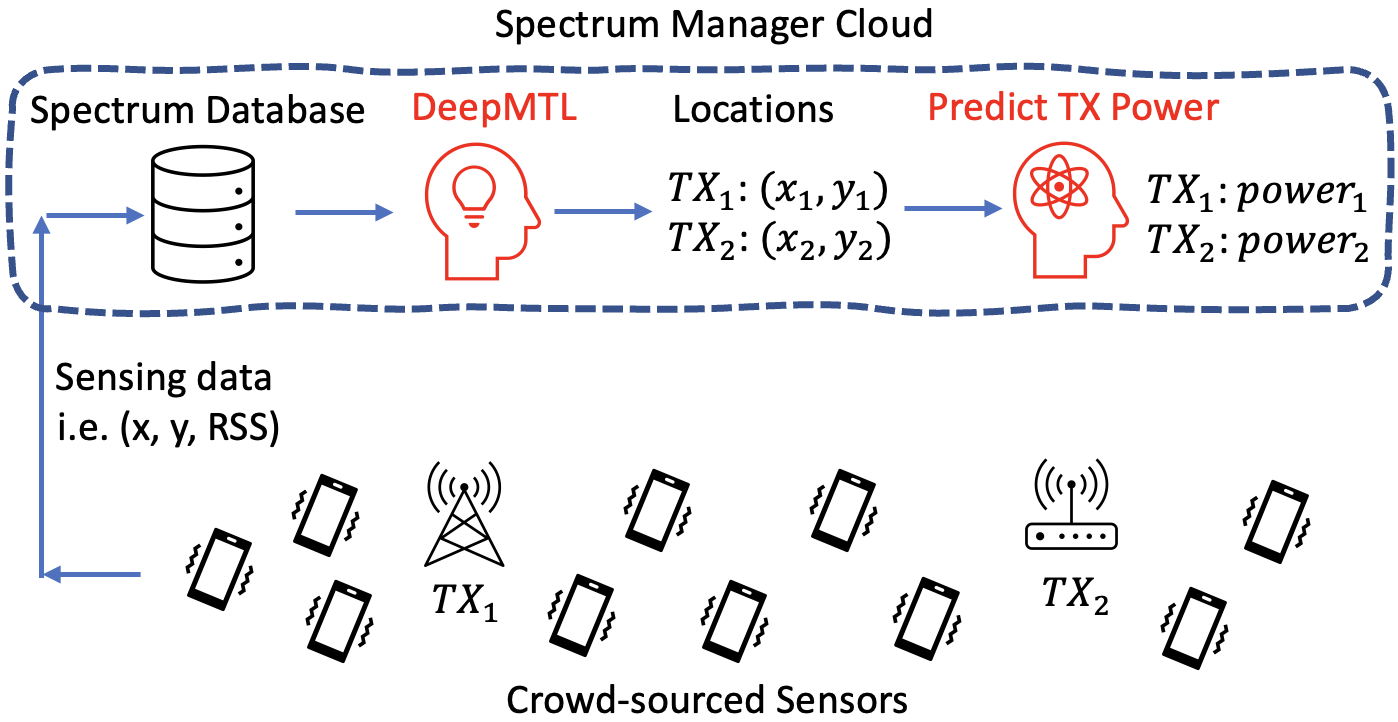
\includegraphics[width=0.9\textwidth]{chapters/wowmom-pmc/figures/architecture.png}
\caption{Multiple transmitter localization using a distributed set of sensors. Sensing data is uploaded to a spectrum manager server in the cloud. \our is a deep learning approach to multiple transmitter localization which helps protect 
spectrum against unauthorized usage. After that, the prediction of transmission powers happens using \our as a building block.}
\label{fig:illustration}
\end{figure}

%%%%%%%WHAT we DO.
\para{\our: Our Two-Step Approach.}  As in prior
works~\cite{mobicom17-splot,chakraborty2017specsense}, we assume a
crowdsourced sensing architecture (See Fig.~\ref{fig:illustration}) wherein relatively low-cost spectrum
sensors are available for gathering signal strength in the form of received power.
We use a convolutional neural network (CNN) based approach
to solve the \mtl problem. In particular, we frame
\mtl as a sequence of two steps: image-to-image translation and object detection, each of which
is solved using a trained CNN model. 
The first step of image-to-image translation maps an input image representing sensor readings to an 
image representing the distribution of transmitter locations, and the second object detection step derives precise
locations of transmitters from the image of transmitter distributions.
We name our \mtl approach as \our.
%%%%%%%%%%%%%%%%%%%

\softpara{Motivation.}
Our overall approach and its various aspects are motivated by the following considerations. 
{\bf First}, we use a learning-based strategy to 
preclude assuming a propagation model~\cite{mobicom17-splot} or conducting surveys of sensors reading distributions~\cite{ipsn20-mtl}.
The assumption of the propagation model suffers from the fact that 
even sophisticated propagation models yield unsatisfactory accuracy and thus lead to degraded performance.
Among all learning-based strategies, deep learning can implicitly capture the environment characteristics (e.g., objects, walls, landscape) in the neural network layers' weights learned through the training of the data~\cite{mobicom20-deeploc}.
Even though a learning-based approach incurs a one-time high training cost,
it generally incurs minimal latency during inference, which is an important consideration for our \mtl problem.
The intruder detection should incur minimal latency to be effective.
{\bf Second}, the geographical nature of the \mtl problem suggests that convolutional neural networks (CNNs) are 
well-suited for efficient
learning of the desired function. In particular, the features of the \mtl problem can be
represented in an image (2D matrix) corresponding to their geographic locations, which can be fed as an input
to an appropriate CNN model that can leverage the spatial correlation among the input features 
to facilitate efficient learning. 
{\bf Lastly,} we use a two-step architecture to facilitate efficient training by essentially
providing an additional intermediate image. 
In particular,  we are able to map each step to well-studied standard computer vision problems, allowing us to build upon known techniques. 

\para{Overall Contributions.}  The goal of our work is to develop an
efficient technique for accurate localization of simultaneously
present multiple transmitters/intruders. We also extend our technique to address various
extensions such as power estimation and the presence of authorized users. Overall, we make the following 
contributions.
\begin{enumerate}
\item
For the \mtl problem, we develop a novel two-step CNN-based approach called \our approach. 
For the first step of image-to-image translation, we develop a CNN model that translates an image representing the sensor readings into an intermediate image that encodes distributions of transmitter locations (Section \ref{sec:translate}). 
%%%%%%%
For the second step of mapping transmitter distributions to precision locations via object detection,
we customize the well-known  object detection method YOLOv3 (Section \ref{sec:detect}).

\item
For localization of transmitters in the presence of authorized users, we 
augment the \our model by adding a pre-processing step based on a 
CNN-model that first reduces the 
sensor readings by the power received from the authorized users (Section \ref{sec:authorized}).

\item
To estimate the transmit power of the intruders, we augment our \our model
with a power-estimation CNN-model which iteratively estimates the power of transmitters
in sub-areas (Section \ref{sec:power}).

\item
We evaluate our techniques via large-scale simulations as well as small-scale testbed data and demonstrate their effectiveness and superior
performance compared to the prior works (Section \ref{sec:evaluation}).
\end{enumerate}

A preliminary version of this paper appeared at IEEE WoWMoM 2021~\cite{wowmom21}.

\eat{ 
\item Why two steps? We could directly go for sensor readings to TX locations .. we help the model by adding an intermediate step.
    
    We aim to fulfill the task by introducing two CNN models. One for converting sensors reading image to TXs image and another one to localize existing TXs.
    The effectiveness of learning-based object localization techniques, in our case, relies on the fact that how accurate and close our representing input (image) is to real objects image. So, we decide, first, to convert sensors reading image to TXs' (real target objects) image via our first CNN model. This way, we block any possible anomaly to propagate to the next CNN model which is a deeper model.
    Another benefit of this approach is to use the output of the first CNN model in non-learning algorithms that may need less training samples (faster) but have probably less accuracy.

}




\eat{
As CNN has proved its powerful strength mostly in Computer Vision and specially in localizing objects in images, sensors being crowd-sourced in a topological area reporting received power from multiple transmitters, representing them as an image will be a natural choice.
The second benefit of training a model is we do not need any knowledge about the signal propagation characteristic.
% Our motivation for using a \map-based
% approach is multifold: First, with sufficient training data, \map is
% known to deliver optimal classification accuracy for the MTL problem.
% Second, the \map approach doesn't assume any propagation model and
% thus works for arbitrary signal propagation characteristics.
Third, relating sensor readings to a TX's image (where TXs are represented as objects based on their location and power) allows us to also estimate the intruder's transmit power, which can be very useful in some applications, e.g., where the penalty is
proportional to the extent of violation.
\blue{Lastly and most importantly,
it naturally extends to being able to handle a presence of an evolving
set of authorized users.}
}


%train convolution  to design a CNN-based model that efficiently localize intruders based on sensors reading. Our approach is a deep learning technique in which sensors reading is represented as CNN-friendly input, an image.


% hypothesis-driven Bayesian approach,
% viz.\ {\em maximum a posteriori} (\map) approach, wherein each
% hypothesis is a configuration (i.e.  a combination of $\langle
% location, power \rangle$ pair) of the potential intruders, and the
% goal is to determine the hypothesis that best explains the sensor
% observations. This determination is done based on the distributions
% (gathered during a training phase) of sensor observations for each
% hypothesis.
%%%%%%%%%%%%


%%%%% MOTIVATION.



% \blue{\emph{Novel Interpolation}. The \map framework requires prior
% training to build probability distributions (PDs) of sensor
% observations for each hypothesis.
% In our work, we reduce the number of PDs to be constructed via a novel
% interpolation scheme suited to our unique setting, and evaluate the
% impact of reduced training on the localization accuracy.}








% 	The RF spectrum is a limited natural resource in great demand. 
	
% 	(Can include a piece of news on US releasing spectrum for 5G from military)
	
% 		%Previous methods using some machine learning techniques are either %not accurate, slow, or not able to localize transmitters close by. 
% 	%Recent work uses deep learning to solve the multiple transmitter %localization problem.
% 	%We utilize the power of convolution neural networks and push the \mtl %solution to the next level.
	
	
% \cite{ipsn20-mtl}
% \cite{mobicom20-deeploc}
% \cite{icccn20-deeptxfinder}